\documentclass[a4paper,10pt]{article}

\usepackage{geometry}
\geometry{
    left=1cm,
    right=1cm,
    bottom=2cm,
    top=2cm
}

\usepackage{tikz}
\usepackage{dblfnote}
\usepackage{lipsum}

\usepackage{xepersian}
\settextfont{Vazirmatn-Regular.ttf}


\title{سوالات احتمالی میان‌ترم 1 درس الگوریتم‌های گراف (با پاسخ)}
\author{استاد مربوطه:\\سرکار خانم دکتر معصومه دامرودی \and به نوشته:\\محمد خورشیدی روزبهانی}
\date{}

\linespread{1.5}

\begin{document}

    \maketitle

    \paragraph{سوال:} تعاریف، قضایا، نتایج و کاربردهای درون اسلایدها را شرح دهید.

    \paragraph{پاسخ:} ابتدا به تعاریف موجود در اسلایدها پرداخته شده و موارد به تفکیک توضیح داده می‌شود.

    \begin{itemize}
        
        \item راس\footnote{\hspace{2pt}Node - Vertex}: راس در گراف نقطه‌ای است که به عنوان یک نقطه یا یک گره شناخته می‌شود و می‌تواند با مقادیر مختلفی مانند عدد صحیح یا رشته مشخص شود.
        
        \item یال\footnote{\hspace{2pt}Edge}: یال در یک گراف، اتصال بین دو راس یا گره است و نشان‌دهنده رابطه بین آن دو راس می‌باشد.
        
        \item در تماس\footnote{\hspace{2pt}Incident}: در مفهوم گراف، هنگامی که یال به یک راس متصل است، می‌گوییم که یال با آن راس «در تماس» است.

        \item گراف ساده\footnote{\hspace{2pt}Graph Simple}: گراف ساده یک گراف است که هیچ یال تکراری یا حلقه‌ای (یالی که شروع و پایانش به یک راس یکسان است) ندارد. به عبارت دیگر، در گراف ساده، هیچ دو راس متصل نیز دوبار در یک یال قرار نمی‌گیرند.
        
        \begin{center}
            
            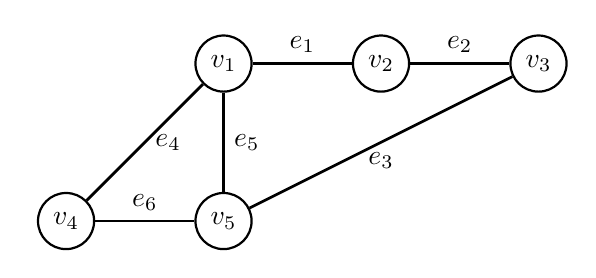
\begin{tikzpicture}
                
                \node[circle, draw, thick] (A) at (-1,2) {$v_1$};
                \node[circle, draw, thick] (B) at (1,2) {$v_2$};
                \node[circle, draw, thick] (C) at (3,2) {$v_3$};
                \node[circle, draw, thick] (D) at (-3,0) {$v_4$};
                \node[circle, draw, thick] (E) at (-1,0) {$v_5$};

                \draw[line width=1pt] (A) -- node[midway, above] {$e_1$} (B);
                \draw[line width=1pt] (A) -- node[midway, right] {$e_5$} (E);
                \draw[line width=1pt] (A) -- node[midway, right] {$e_4$} (D);
                \draw[line width=1pt] (B) -- node[midway, above] {$e_2$} (C);
                \draw[line width=1pt] (C) -- node[midway, below] {$e_3$} (E);
                \draw[line width=1pt] (D) -- node[midway, above] {$e_6$} (E);

            \end{tikzpicture}

        \end{center}
        
        \item درجه\footnote{\hspace{2pt}Degree}: درجه یک راس در گراف، تعداد یال‌های متصل به آن راس است. به عبارت دیگر، درجه یک راس نشان‌دهنده تعداد یال‌هایی است که به آن راس متصل هستند.
        
        \item راس منفرد\footnote{\hspace{2pt}Vertex Isolated}: راس منفرد یک راس در گراف است که هیچ یالی به آن متصل نیست، به عبارت دیگر درجه این راس صفر است.
        
        \item متمم\footnote{\hspace{2pt}Complement}: در مفهوم گراف، متمم یک گراف، گرافی است که همه یال‌های موجود در گراف اصلی حذف شده و همه یال‌هایی که بین رئوس موجود نیستند اضافه شده‌اند. به عبارت دیگر، این گراف حاصل از دو گراف اصلی که هیچ یال مشترکی ندارند می‌باشد.
        
        \begin{center}
            
            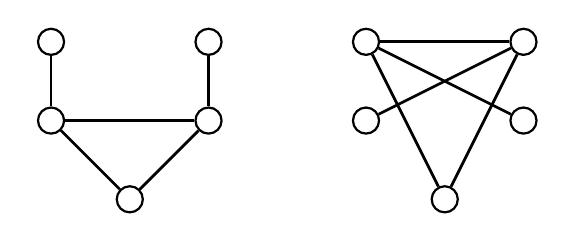
\begin{tikzpicture}
                
                \node[circle, draw, thick] (A) at (-5,0) {};
                \node[circle, draw, thick] (B) at (-3,0) {};
                \node[circle, draw, thick] (C) at (-5,-1) {};
                \node[circle, draw, thick] (D) at (-3,-1) {};
                \node[circle, draw, thick] (E) at (-4,-2) {};

                \draw[line width=1pt] (A) -- (C);
                \draw[line width=1pt] (B) -- (D);
                \draw[line width=1pt] (C) -- (D);
                \draw[line width=1pt] (D) -- (E);
                \draw[line width=1pt] (C) -- (E);

                \node[circle, draw, thick] (F) at (-1,0) {};
                \node[circle, draw, thick] (G) at (1,0) {};
                \node[circle, draw, thick] (H) at (-1,-1) {};
                \node[circle, draw, thick] (I) at (1,-1) {};
                \node[circle, draw, thick] (J) at (0,-2) {};

                \draw[line width=1pt] (F) -- (J);
                \draw[line width=1pt] (G) -- (J);
                \draw[line width=1pt] (F) -- (G);
                \draw[line width=1pt] (G) -- (H);
                \draw[line width=1pt] (F) -- (I);

            \end{tikzpicture}

        \end{center}

        \item گراف خالی\footnote{\hspace{2pt}Graph Empty}: گراف  خالی یک گراف است که هیچ راس و هیچ یالی ندارد. به عبارت دیگر، یک گراف با تعداد رئوس و یال‌های صفر است.

        \item زیرگراف\footnote{\hspace{2pt}Subgraph}: زیرگراف یک گراف است که تمام رئوس و یال‌های آن در گراف اصلی وجود داشته باشند. به عبارت دیگر، اگر یک گراف با رئوس و یال‌های خاصی را در نظر بگیرید، هر گرافی که شامل زیرمجموعه‌ای ار آن رئوس و یال‌ها باشد، زیرگرافی از آن گراف است.
        
        \begin{center}
                    
            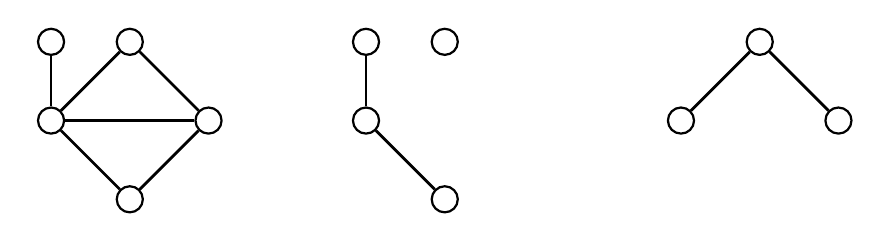
\begin{tikzpicture}
                
                \node[circle, draw, thick] (A) at (-1,0) {};
                \node[circle, draw, thick] (B) at (-1,-1) {};
                \node[circle, draw, thick] (C) at (0,0) {};
                \node[circle, draw, thick] (D) at (1,-1) {};
                \node[circle, draw, thick] (E) at (0,-2) {};

                \draw[line width=1pt] (A) -- (B);
                \draw[line width=1pt] (B) -- (C);
                \draw[line width=1pt] (C) -- (D);
                \draw[line width=1pt] (D) -- (E);
                \draw[line width=1pt] (E) -- (B);
                \draw[line width=1pt] (B) -- (D);

                \node[circle, draw, thick] (A) at (3,0) {};
                \node[circle, draw, thick] (B) at (3,-1) {};
                \node[circle, draw, thick] (C) at (4,0) {};
                \node[circle, draw, thick] (E) at (4,-2) {};

                \draw[line width=1pt] (A) -- (B);
                \draw[line width=1pt] (E) -- (B);

                \node[circle, draw, thick] (B) at (7,-1) {};
                \node[circle, draw, thick] (C) at (8,0) {};
                \node[circle, draw, thick] (D) at (9,-1) {};

                \draw[line width=1pt] (B) -- (C);
                \draw[line width=1pt] (C) -- (D);

            \end{tikzpicture}

        \end{center}

        \item گراف صفر\footnote{\hspace{2pt}Graph Null}: گراف صفر یک گراف است که تنها یک راس دارد و هیچ یالی ندارد.

        \item گراف کامل\footnote{\hspace{2pt}Graph Complete}: یک گراف است که همه رئوس آن به همه رئوس دیگر با یک یال متصل هستند. به عبارت دیگر، در یک گراف کامل هیچ دو راسی وجود ندارد که بهم هم متصصل نباشند.
        
        \begin{center}
                        
            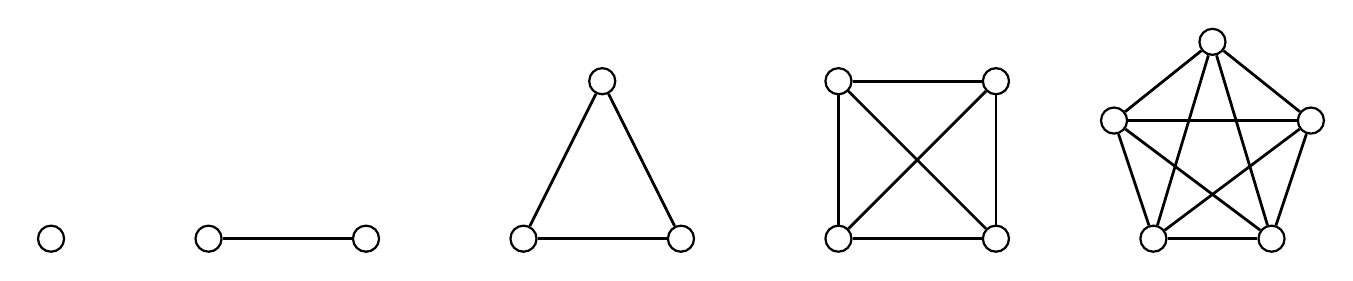
\begin{tikzpicture}
                
                \node[circle, draw, thick] (A) at (0,-4) {};

                \node[circle, draw, thick] (B) at (2,-4) {};
                \node[circle, draw, thick] (C) at (4,-4) {};

                \draw[line width=1pt] (B) -- (C);

                \node[circle, draw, thick] (D) at (7,-2) {};
                \node[circle, draw, thick] (E) at (6,-4) {};
                \node[circle, draw, thick] (F) at (8,-4) {};

                \draw[line width=1pt] (D) -- (E);
                \draw[line width=1pt] (E) -- (F);
                \draw[line width=1pt] (F) -- (D);

                \node[circle, draw, thick] (G) at (10,-2) {};
                \node[circle, draw, thick] (H) at (12,-2) {};
                \node[circle, draw, thick] (I) at (12,-4) {};
                \node[circle, draw, thick] (J) at (10,-4) {};

                \draw[line width=1pt] (G) -- (H);
                \draw[line width=1pt] (H) -- (I);
                \draw[line width=1pt] (I) -- (J);
                \draw[line width=1pt] (J) -- (G);
                \draw[line width=1pt] (G) -- (I);
                \draw[line width=1pt] (H) -- (J);

                \node[circle, draw, thick] (K) at (14.75,-1.5) {};
                \node[circle, draw, thick] (L) at (16,-2.5) {};
                \node[circle, draw, thick] (M) at (14,-4) {};
                \node[circle, draw, thick] (N) at (15.5,-4) {};
                \node[circle, draw, thick] (O) at (13.5,-2.5) {};

                \draw[line width=1pt] (K) -- (L);
                \draw[line width=1pt] (K) -- (M);
                \draw[line width=1pt] (K) -- (N);
                \draw[line width=1pt] (K) -- (O);
                \draw[line width=1pt] (L) -- (M);
                \draw[line width=1pt] (L) -- (N);
                \draw[line width=1pt] (L) -- (O);
                \draw[line width=1pt] (M) -- (N);
                \draw[line width=1pt] (M) -- (O);
                \draw[line width=1pt] (N) -- (O);

            \end{tikzpicture}

        \end{center}

        \item گراف :k-منتظم\footnote{\hspace{2pt}Graph k-Regular} گراف k-منتظم یک گراف است که درجه همه رئوس آن برابر با k باشد. به عبارت دیگر، هر راس در این گراف، با k یال به راس‌های دیگر متصل است.
        
        \begin{center}
                        
            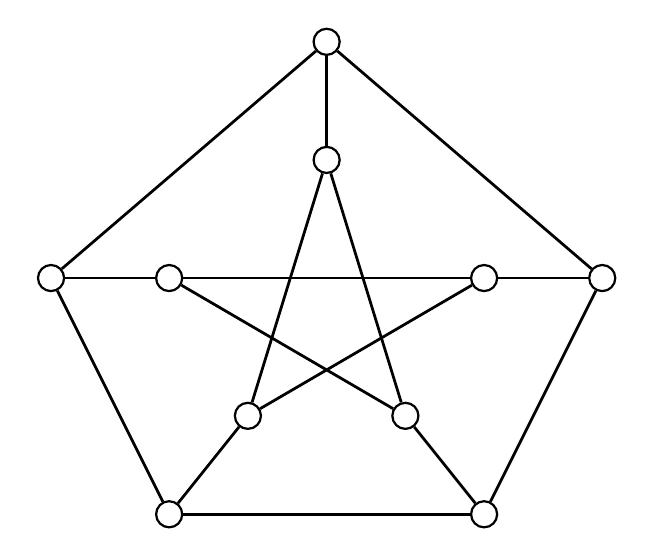
\begin{tikzpicture}
                
                \node[circle, draw, thick] (A) at (0,0) {};
                \node[circle, draw, thick] (B) at (3.5,-3) {};
                \node[circle, draw, thick] (C) at (2,-6) {};
                \node[circle, draw, thick] (D) at (-2,-6) {};
                \node[circle, draw, thick] (E) at (-3.5,-3) {};
                \node[circle, draw, thick] (F) at (0,-1.5) {};
                \node[circle, draw, thick] (G) at (2,-3) {};
                \node[circle, draw, thick] (H) at (1,-4.75) {};
                \node[circle, draw, thick] (I) at (-1,-4.75) {};
                \node[circle, draw, thick] (J) at (-2,-3) {};

                \draw[line width=1pt] (A) -- (B);
                \draw[line width=1pt] (B) -- (C);
                \draw[line width=1pt] (C) -- (D);
                \draw[line width=1pt] (D) -- (E);
                \draw[line width=1pt] (E) -- (A);
                \draw[line width=1pt] (A) -- (F);
                \draw[line width=1pt] (B) -- (G);
                \draw[line width=1pt] (C) -- (H);
                \draw[line width=1pt] (D) -- (I);
                \draw[line width=1pt] (E) -- (J);
                \draw[line width=1pt] (F) -- (H);
                \draw[line width=1pt] (F) -- (I);
                \draw[line width=1pt] (G) -- (I);
                \draw[line width=1pt] (G) -- (J);
                \draw[line width=1pt] (H) -- (J);

            \end{tikzpicture}

        \end{center}

        \item چرخه\footnote{\hspace{2pt}Graph Circuit - Graph Cycle}: در مفهوم گراف، چرخه یک مسیر بسته است که از یک راس شروع شده، از یال‌های مختلف گذر کرده و در نهایت به همان راس اول باز می‌گردد. به عبارت دیگر، یک چرخه گرافی که شامل حداقل یک راس و حداقل یک یال است و اولین و آخرین راس‌ها یکسان هستند.
        
        \begin{center}
            
            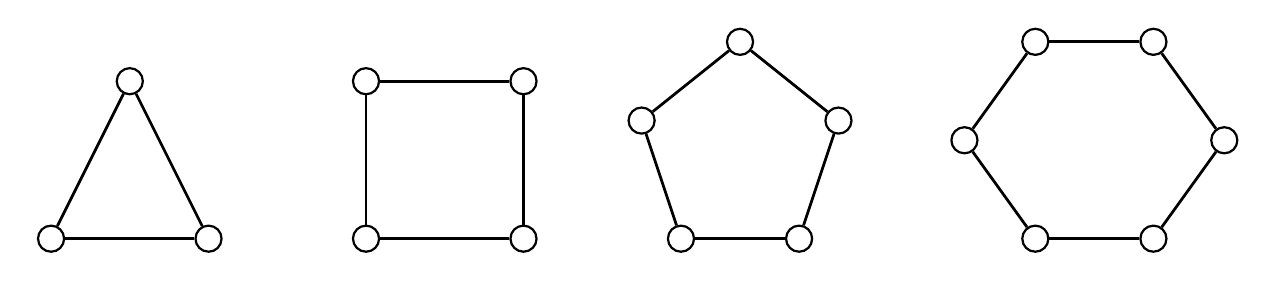
\begin{tikzpicture}
                
                \node[circle, draw, thick] (D) at (7,-2) {};
                \node[circle, draw, thick] (E) at (6,-4) {};
                \node[circle, draw, thick] (F) at (8,-4) {};

                \draw[line width=1pt] (D) -- (E);
                \draw[line width=1pt] (E) -- (F);
                \draw[line width=1pt] (F) -- (D);

                \node[circle, draw, thick] (G) at (10,-2) {};
                \node[circle, draw, thick] (H) at (12,-2) {};
                \node[circle, draw, thick] (I) at (12,-4) {};
                \node[circle, draw, thick] (J) at (10,-4) {};

                \draw[line width=1pt] (G) -- (H);
                \draw[line width=1pt] (H) -- (I);
                \draw[line width=1pt] (I) -- (J);
                \draw[line width=1pt] (J) -- (G);

                \node[circle, draw, thick] (K) at (14.75,-1.5) {};
                \node[circle, draw, thick] (L) at (16,-2.5) {};
                \node[circle, draw, thick] (M) at (14,-4) {};
                \node[circle, draw, thick] (N) at (15.5,-4) {};
                \node[circle, draw, thick] (O) at (13.5,-2.5) {};

                \draw[line width=1pt] (K) -- (L);
                \draw[line width=1pt] (L) -- (N);
                \draw[line width=1pt] (M) -- (N);
                \draw[line width=1pt] (M) -- (O);
                \draw[line width=1pt] (O) -- (K);

                \node[circle, draw, thick] (P) at (18.5,-1.5) {};
                \node[circle, draw, thick] (Q) at (20,-1.5) {};
                \node[circle, draw, thick] (R) at (20.9,-2.75) {};
                \node[circle, draw, thick] (S) at (20,-4) {};
                \node[circle, draw, thick] (T) at (18.5,-4) {};
                \node[circle, draw, thick] (U) at (17.6,-2.75) {};

                \draw[line width=1pt] (P) -- (Q);
                \draw[line width=1pt] (Q) -- (R);
                \draw[line width=1pt] (R) -- (S);
                \draw[line width=1pt] (S) -- (T);
                \draw[line width=1pt] (T) -- (U);
                \draw[line width=1pt] (U) -- (P);

            \end{tikzpicture}

        \end{center}

        \item گراف چرخ\footnote{\hspace{2pt}Graph Wheel}: در مفهوم گراف یک گراف چرخ یک نوع خاص از گراف است که از راس مرکزی و چندین راس دیگر تشکیل شده است که همگی به راس مرکزی متصل هستند و هیچ یالی بین رئوس غیرمرکزیِ غیرمجاور وجود ندارد. به عبارت دیگر، یک گراف چرخ همانند گراف چرخه است با این تفاوت که یک راس به عنوان مرکز در نظر گرفته می‌شود و همه رئوس دیگر به آن متصل می‌شوند.
        
        \begin{center}
            
            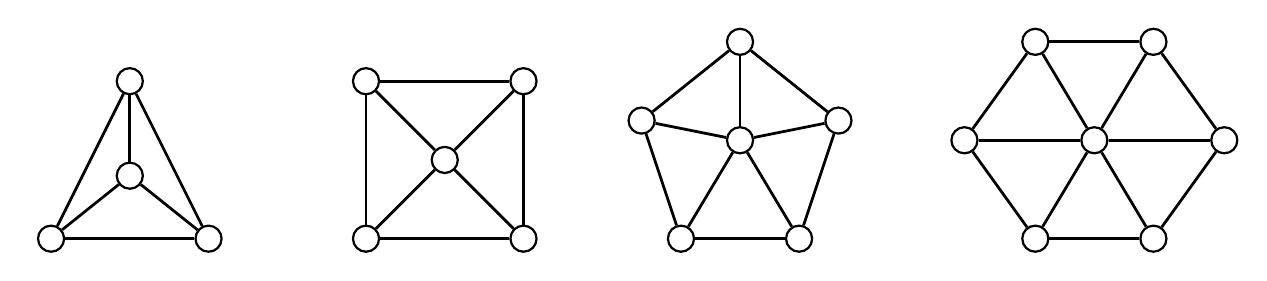
\begin{tikzpicture}
                
                \node[circle, draw, thick] (D) at (7,-2) {};
                \node[circle, draw, thick] (E) at (6,-4) {};
                \node[circle, draw, thick] (F) at (8,-4) {};
                \node[circle, draw, thick] (W) at (7,-3.2) {};

                \draw[line width=1pt] (D) -- (E);
                \draw[line width=1pt] (E) -- (F);
                \draw[line width=1pt] (F) -- (D);
                \draw[line width=1pt] (D) -- (W);
                \draw[line width=1pt] (E) -- (W);
                \draw[line width=1pt] (F) -- (W);

                \node[circle, draw, thick] (G) at (10,-2) {};
                \node[circle, draw, thick] (H) at (12,-2) {};
                \node[circle, draw, thick] (I) at (12,-4) {};
                \node[circle, draw, thick] (J) at (10,-4) {};
                \node[circle, draw, thick] (X) at (11,-3) {};

                \draw[line width=1pt] (G) -- (H);
                \draw[line width=1pt] (H) -- (I);
                \draw[line width=1pt] (I) -- (J);
                \draw[line width=1pt] (J) -- (G);
                \draw[line width=1pt] (G) -- (X);
                \draw[line width=1pt] (H) -- (X);
                \draw[line width=1pt] (I) -- (X);
                \draw[line width=1pt] (J) -- (X);

                \node[circle, draw, thick] (K) at (14.75,-1.5) {};
                \node[circle, draw, thick] (L) at (16,-2.5) {};
                \node[circle, draw, thick] (M) at (14,-4) {};
                \node[circle, draw, thick] (N) at (15.5,-4) {};
                \node[circle, draw, thick] (O) at (13.5,-2.5) {};
                \node[circle, draw, thick] (Y) at (14.75,-2.75) {};

                \draw[line width=1pt] (K) -- (L);
                \draw[line width=1pt] (L) -- (N);
                \draw[line width=1pt] (M) -- (N);
                \draw[line width=1pt] (M) -- (O);
                \draw[line width=1pt] (O) -- (K);
                \draw[line width=1pt] (K) -- (Y);
                \draw[line width=1pt] (L) -- (Y);
                \draw[line width=1pt] (M) -- (Y);
                \draw[line width=1pt] (N) -- (Y);
                \draw[line width=1pt] (O) -- (Y);

                \node[circle, draw, thick] (P) at (18.5,-1.5) {};
                \node[circle, draw, thick] (Q) at (20,-1.5) {};
                \node[circle, draw, thick] (R) at (20.9,-2.75) {};
                \node[circle, draw, thick] (S) at (20,-4) {};
                \node[circle, draw, thick] (T) at (18.5,-4) {};
                \node[circle, draw, thick] (U) at (17.6,-2.75) {};
                \node[circle, draw, thick] (Z) at (19.25,-2.75) {};

                \draw[line width=1pt] (P) -- (Q);
                \draw[line width=1pt] (Q) -- (R);
                \draw[line width=1pt] (R) -- (S);
                \draw[line width=1pt] (S) -- (T);
                \draw[line width=1pt] (T) -- (U);
                \draw[line width=1pt] (U) -- (P);
                \draw[line width=1pt] (P) -- (Z);
                \draw[line width=1pt] (Q) -- (Z);
                \draw[line width=1pt] (R) -- (Z);
                \draw[line width=1pt] (S) -- (Z);
                \draw[line width=1pt] (T) -- (Z);
                \draw[line width=1pt] (U) -- (Z);


            \end{tikzpicture}

        \end{center}
        
        \item گراف مکعب n بُعدی\footnote{\hspace{2pt}Graph n-Cube}: در مفهوم گراف، مکعب n بُعدی یک گراف با ساختار مکعبی است که دارای $n^2$ راس و $n \times (n-1)^2$ یال است. این گراف معمولاً با استفاده از ارقام دودویی به عنوان برچسب رئوس تعریف می‌شود، به طوری که هر راس با یک دنباله n بیتی نمایش داده می‌شود و هر یال به دو راس متصل است که دنباله‌های باینری متفاوت در یک بیت داشته باشند.
        
        \begin{center}
            
            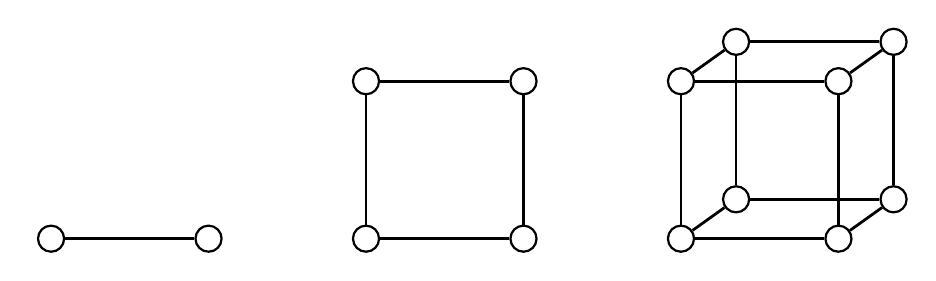
\begin{tikzpicture}
                
                \node[circle, draw, thick] (A) at (0,0) {};
                \node[circle, draw, thick] (B) at (2,0) {};

                \draw[line width=1pt] (A) -- (B);

                \node[circle, draw, thick] (A) at (4,2) {};
                \node[circle, draw, thick] (B) at (6,2) {};
                \node[circle, draw, thick] (C) at (6,0) {};
                \node[circle, draw, thick] (D) at (4,0) {};

                \draw[line width=1pt] (A) -- (B);
                \draw[line width=1pt] (B) -- (C);
                \draw[line width=1pt] (C) -- (D);
                \draw[line width=1pt] (D) -- (A);

                \node[circle, draw, thick] (A) at (8,2) {};
                \node[circle, draw, thick] (B) at (10,2) {};
                \node[circle, draw, thick] (C) at (10,0) {};
                \node[circle, draw, thick] (D) at (8,0) {};

                \node[circle, draw, thick] (E) at (8.7,2.5) {};
                \node[circle, draw, thick] (F) at (10.7,2.5) {};
                \node[circle, draw, thick] (G) at (10.7,0.5) {};
                \node[circle, draw, thick] (H) at (8.7,0.5) {};

                \draw[line width=1pt] (A) -- (B);
                \draw[line width=1pt] (B) -- (C);
                \draw[line width=1pt] (C) -- (D);
                \draw[line width=1pt] (D) -- (A);

                \draw[line width=1pt] (A) -- (E);
                \draw[line width=1pt] (B) -- (F);
                \draw[line width=1pt] (C) -- (G);
                \draw[line width=1pt] (D) -- (H);

                \draw[line width=1pt] (E) -- (F);
                \draw[line width=1pt] (F) -- (G);
                \draw[line width=1pt] (G) -- (H);
                \draw[line width=1pt] (H) -- (E);


            \end{tikzpicture}

        \end{center}
        
        \item گراف مسیر\footnote{\hspace{2pt}Graph Path}: گراف مسیر یک گراف است که رئوس آن به صورت متوالی به هم متصل هستند و هیچ یال تکراری یا حلقه‌ای وجود ندارد. به عبارت دیگر، این گراف مانند زنجیره است که رئوس آن به ترتیب به یکدیگر متصل شده‌اند.
        
        \begin{center}
            
            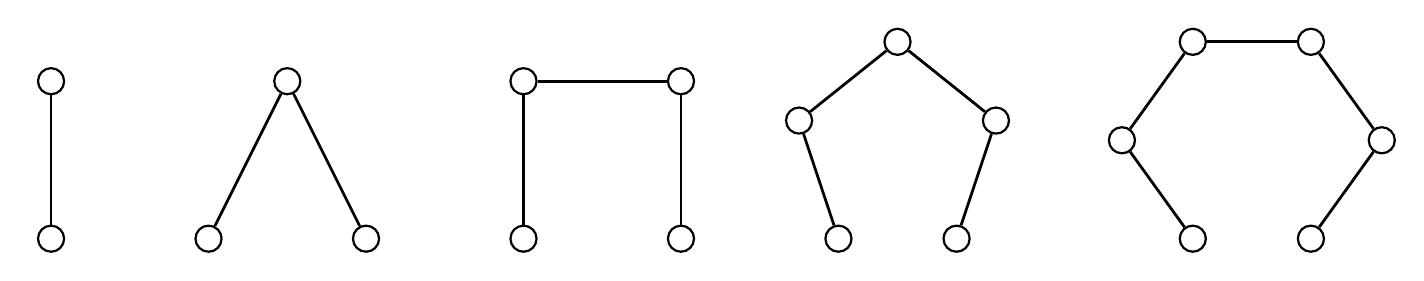
\begin{tikzpicture}

                \node[circle, draw, thick] (A) at (4,-2) {};
                \node[circle, draw, thick] (B) at (4,-4) {};

                \draw[line width=1pt] (A) -- (B);
                
                \node[circle, draw, thick] (D) at (7,-2) {};
                \node[circle, draw, thick] (E) at (6,-4) {};
                \node[circle, draw, thick] (F) at (8,-4) {};

                \draw[line width=1pt] (D) -- (E);
                \draw[line width=1pt] (F) -- (D);

                \node[circle, draw, thick] (G) at (10,-2) {};
                \node[circle, draw, thick] (H) at (12,-2) {};
                \node[circle, draw, thick] (I) at (12,-4) {};
                \node[circle, draw, thick] (J) at (10,-4) {};

                \draw[line width=1pt] (G) -- (H);
                \draw[line width=1pt] (H) -- (I);
                \draw[line width=1pt] (J) -- (G);

                \node[circle, draw, thick] (K) at (14.75,-1.5) {};
                \node[circle, draw, thick] (L) at (16,-2.5) {};
                \node[circle, draw, thick] (M) at (14,-4) {};
                \node[circle, draw, thick] (N) at (15.5,-4) {};
                \node[circle, draw, thick] (O) at (13.5,-2.5) {};

                \draw[line width=1pt] (K) -- (L);
                \draw[line width=1pt] (L) -- (N);
                \draw[line width=1pt] (M) -- (O);
                \draw[line width=1pt] (O) -- (K);

                \node[circle, draw, thick] (P) at (18.5,-1.5) {};
                \node[circle, draw, thick] (Q) at (20,-1.5) {};
                \node[circle, draw, thick] (R) at (20.9,-2.75) {};
                \node[circle, draw, thick] (S) at (20,-4) {};
                \node[circle, draw, thick] (T) at (18.5,-4) {};
                \node[circle, draw, thick] (U) at (17.6,-2.75) {};

                \draw[line width=1pt] (P) -- (Q);
                \draw[line width=1pt] (Q) -- (R);
                \draw[line width=1pt] (R) -- (S);
                \draw[line width=1pt] (T) -- (U);
                \draw[line width=1pt] (U) -- (P);



            \end{tikzpicture}

        \end{center}

        \item گراف بازه\footnote{\hspace{2pt}Graph Interval}: گراف بازه یک نوع خاص از گراف است که رئوس آن بازه‌های اعداد حقیقی را نمایش می‌دهند و دو راس متصل هستند اگر و تنها اگر بازه‌های متناظر با آن دو راس تلاقی داشته باشند. به عبارت دیگر، گراف بازه می‌تواند به عنوان نمایشی از یک مجموعهٔ بازه‌های اعداد حقیقی دیده شود، که هر گره نمایانگر یک بازه است و یال بین دو گره وجود دارد اگر و تنها اگر بازه‌های متناظر با آن دو گره تلاقی داشته باشند.
        
        \item گراف قوس دایره‌ای\footnote{\hspace{2pt}Graph Circular-arc}: گراف قوس دایره‌ای، یک نوع خاص از گراف است که رئوس آن بازه‌های یک دایره را نمایش می‌دهند و دو راس متصل هستند اگر و تنها اگر بازه‌های متناظر با آن دو راس اشتراک غیرخالی داشته باشند. به عبارت دیگر، گراف قوس دایره‌ای می‌تواند به عنوان نمایشی از بازه‌های یک دایره دیده شود، که هر راس نمایانگر یک بازه است و دو راس متصل هستند اگر و تنها اگر بازه‌های متناظر با آن دو راس اشتراک غیرخالی داشته باشند.
        
        \item گراف دوبخشی\footnote{\hspace{2pt}Graph Bipartite}: گراف دوبخشی یک گراف است که مجموعه رئوس آن را می‌توان به دو زیرمجموعه جدا از هم تقسیم کرد، به طوری که هیچ راس درون هر زیرمجموعه با راسی در همان زیرمجموعه دیگر متصل نباشد. به عبارت دیگر، این گراف متشکل از دو مجموعه راس است که هر یال تنها بین یک راس از یک مجموعه و یک راس از مجموعه دیگر وجود دارد، نه دو راس از همان مجموعه.

        \item گراف دوبخشی کامل\footnote{\hspace{2pt}Graph Bipartite Complete}: گراف دوبخشی کامل یک گراف دوبخشی است که همه رئوس یک زیرمجموعه با همه رئوس زیرمجموعه دیگر به صورت کامل متصل هستند. به عبارت دیگر، هر راس در یک زیرمجموعه با همه راس‌های زیرمجموعه دیگر متصل است.
        
        \item پیاده‌روی\footnote{\hspace{2pt}Walk}: در مفهوم گراف، پیاده‌روی یک دنباله از رئوس و یال‌ها است که از یک راس شروع شده و در آن رئوس و یال‌ها به ترتیب دنبال می‌شوند، به طوری که هر راس در مسیر با یک یال به راس بعدی متصل باشد. به عبارت دیگر، پیاده‌روی می‌تواند شامل تکرار یال‌ها و رئوس باشد.
        
        \item مسیر\footnote{\hspace{2pt}Trail}: در مفهوم گراف، مسیر یک دنباله از یال‌ها و رئوس است که هر یال در آن فقط یک بار ظاهر شده ولی رئوس ممکن است چندین بار ظاهر شوند. به عبارت دیگر، یک مسیر یک پیاده‌روی است که هیچ یال تکراری ندارد.

        \item مسیر\footnote{\hspace{2pt}Path}: در مفهوم گراف، مسیر یک دنباله از رئوس است که هر راس در آن با ییکک یال به راس بعدی متصل است. به عبارت دیگر، این یک زنجیره از رئوس است که هیچ راس تکراری ندارد.
        
        \item چرخه\footnote{\hspace{2pt}Cycle}: در مفهوم گراف، چرخه یک مسیر بسته است که از یک راس شروع شده و در آن رئوس و یال‌ها به ترتیب دنبال می‌شوند، به طوری که آخرین راس به راس اولیه باز می‌گردد. به عبارت دیگر، این یک مسیر است که همچنین به عنوان یک چرخه شناخته می‌شود.

        \item بسته\footnote{\hspace{2pt}Closed}: در مفهوم گراف، اصطلاح «بسته» ممکن است به مسیرها یا چرخه‌هایی اشاره کند که یک نقطه شروع و پایان مشترک دارند و بنابراین «بسته» نامیده می‌شوند. به طوری که برای مسیرها، می‌توان آن‌ها را مسیرهای بسته\footnote{\hspace{2pt}Paths Closed} نامید و برای چرخه‌ها، آن‌ها را چرخه‌های بسته\footnote{\hspace{2pt}Cycles Closed} نامید.
        
        \item گراف جهت‌دار\footnote{\hspace{2pt}Digraph - Graph Directed}: گراف جهت‌دار یک گراف است که هر یال آن یک جهت خاص دارد. به عبارت دیگر، یال‌ها دارای جهتی هستند و معمولاً به عنوان یک جفت از رئوس نمایش داده می‌شوند، به عنوان مثال، اگر یالی از راس A به راس B وجود داشته باشد، این به معنای این است که می‌توان از راس A به راس B حرکت کرد ولی ممکن نیست بتوان از راس B به راس A حرکت کرد.
        
        \item منبع\footnote{\hspace{2pt}Source}: در یک گراف جهت‌دار، راسی که هیچ یالی وارد آن نیست، منبع نامیده می‌شود. به عبارت دیگر، منبع راسی است که فقط یال‌هایی از آن خارج می‌شود.
        
        \item ترمینال\footnote{\hspace{2pt}Terminal}: در یک گراف جهت‌دار، راسی که هیچ یالی از آن خارج نمی‌شود، ترمینال نامیده می‌شود. به عبارت دیگر، ترمینال راسی است که فقط یال‌هایی به آن وارد می‌شود.
        
        \item درجه ورودی\footnote{\hspace{2pt}in-Degree}: در یک گراف جهت‌دار، درجه‌ی ورودی یک راس، تعداد یال‌هایی است که به آن راس وارد می‌شوند.
        
        \item درجه خروجی\footnote{\hspace{2pt}out-Degree}: در یک گراف جهت‌دار، درجه‌ی خروجی یک راس، تعداد یال‌هایی است که از آن راس خارج می‌شوند.

        \item متعادل بودن\footnote{\hspace{2pt}Balanced}: در مفهوم گراف جهت‌دار، یک مفهوم مرتبط با مسیرهای آن، مفهوم متعادل بودن است. یک مسیر متعادل، مسیری است که برای هر راس، تعداد یال‌هایی که وارد آن می‌شوند، با تعداد یال‌هایی که از آن خارج می‌شوند، برابر است. به عبارت دیگر، درجه ورودی هر راس با درجه خروجی آن برابر است.
        
        \item پیش‌ران\footnote{\hspace{2pt}Predecessor}: در مفهوم گراف جهت‌دار، پیش‌ران یک راس، راس‌هایی هستند که یال‌هایی به این راس می‌رسند، به عبارت دیگر، رئوسی که به این راس متصل هستند و در جهتی عکس جهت یال‌ها به آن می‌روند.

        \item ماتریس مجاورت\footnote{\hspace{2pt}Matrix Adjacency}: ماتریس مجاورت یک نمایش گراف است که در آن رئوس به عنوان ردیف‌ها و ستون‌ها نمایش داده می‌شوند و وجود یا عدم وجود یال بین هر دو راس با استفاده از مقادیر درون ماتریس نشان داده می‌شود. اگر گراف جهت‌دار باشد، معمولاً ماتریس مجاورت برای نمایش جهات یال‌ها از مقادیر 0 و 1 استفاده می‌کند؛ به این معنی که یک مقدار 1 در موقعیت $(i, j)$ نشان دهنده وجود یال از راس $i$ به راس $j$ است، در حالی که مقدار 0 نشان‌دهنده عدم وجود یال است. در صورتی که گراف جهت‌دار نباشد، این مقادیر ممکن است به صورت متقارن باشند.
        
        \item تلاقی\footnote{\hspace{2pt}Incidence}: در مفهوم گراف، تلاقی به ارتباط بین رئوس و یال‌ها اشاره دارد. به عبارت دیگر، ارتباط میان رئوس و یال‌هایی که این رئوس را به هم متصل می‌کنند. در یک گراف جهت‌دار، تلاقی ممکن است به جهت یال‌ها نیز اشاره داشته باشد، به این معنی که مشخص می‌کند که کدام رأس به عنوان منبع و کدام رأس به عنوان ترمینال یک یال در نظر گرفته می‌شود.
        
        \item ماتریس پراکنده\footnote{\hspace{2pt}Matrix Sparse}: ماتریس پراکنده یک نوع ماتریس است که در آن اکثریت عناصر آن صفر هستند. این نوع ماتریس برای نمایش داده‌هایی که اکثر مقادیر آن‌ها صفر هستند، مفید است، زیرا ذخیره‌سازی بهینه‌تری نسبت به ماتریس معمولی دارد.
        
        \item گراف‌های ایزومرفیک\footnote{\hspace{2pt}Graphs Isomorphic}: گراف‌های ایزومرفیک دو گراف هستند که در یکدیگر قابل تبدیل باشند. به عبارت دیگر، اگر بتوان هر یک از آن‌ها را با تغییر نام رئوس به یکدیگر تبدیل کرد به طوری که ساختار یال‌ها و اتصالات میان رئوس حفظ شود، آنگاه این دو گراف ایزومرفیک هستند. به عبارت دیگر، این دو گراف در واقع «همان» گراف هستند و تنها نامگذاری رئوس آن‌ها متفاوت است.
        
        \item زیرگراف ایزومرفیک\footnote{\hspace{2pt}Isomorphism Subgraph}: در مفهوم گراف، زیرگراف ایزومرفیک زمانی رخ می‌دهد که یک گراف (زیرگراف) دیگری را به صورت زیرگراف در خود جای دهد. به عبارت دیگر، اگر یک گراف (زیرگراف کوچک‌تر) وجود داشته باشد که در گراف دیگر (زیرگراف بزرگ‌تر) به صورت زیرگراف جای بگیرد، آنگاه این دو گراف زیرگراف ایزومرفیک هستند.

    \end{itemize}

    اکنون به قضایا و نتایج درون اسلایدها پرداخته می‌شود و موارد به تفکیک توضیح داده می‌شود.

    \begin{itemize}
        
        \item مجموع درجات یک گراف $G=(V,E)$ برابر است با $2|E|=2m$.
        
        \item تعداد رئوسی که درجه آن‌ها فرد است، زوج می‌باشد.

        \item گراف کامل $K_n$ با گراف منتظم-$n-1$ برابر است.

        \item یک پیاده‌روی از $u$ به یک $v$ (به صورتی که $u \neq v$) حاوی مسیری از $u$ به $v$ است. (نکته: حذف چرخه‌های فرعی)

        \item یک پیاده‌روی بسته با طول فرد شامل چرخه‌ای از طول فرد است.

        \item در گراف جهت‌دار، هر گراف بدون دور\footnote{\hspace{2pt}Graph Acyclic} حداقل یک راس دارد که درجه ورودی آن برابر صفر باشد.

        \item تعداد پیاده‌روی‌های به طول $k$ از راس $i$ تا راس $j$ برابر است با $A^k_{ij}$

        \item اگر تابع اثر یک ماتریس نشان‌دهنده مجموع درایه‌های قطر اصلی ماتریس باشد، آنگاه در گراف‌های بدون جهت داریم که:
        
            \begin{itemize}
                
                \item مجموع درایه‌های قطر اصلیِ ماتریس مجاورت برابر صفر می‌باشد. به عبارت دیگر $tr(A)=0$ برقرار است.
                
                \item مجموع درایه‌های قطر اصلیِ توان دوم ماتریس مجاورت، دو برابر تعداد یال‌ها می‌باشد. به عبارت دیگر $tr(A^2)=2|E|$ برقرار است.
                
                \item مجموع درایه‌های قطر اصلیِ توان سوم ماتریس مجاورت، شش برابر تعداد مثلث‌های موجود در گراف می‌باشد. به عبارت دیگر $tr(A^3)=the \hspace{3pt} number \hspace{3pt} of \hspace{3pt} triangles \hspace{3pt} in \hspace{3pt} graph$ برقرار است.

            \end{itemize}

    \end{itemize}

    اکنون به کاربردهای دورن اسلایدها پرداخته می‌شود و موراد به تفکیک توضیح داده می‌شود.

    \begin{itemize}
        
        \item کاربردهای گراف بازه‌ای:
        
        \begin{itemize}

            \item مدل کردن مسائل دنیای واقعی با ساختار ریاضی
            
            \item زمان‌بندی رویدادهای مختلف و مدیریت تداخل‌های زمانی
            
            \item نقشه برداری DNA

            \item نحوه تنظیم دمای یخچال‌های آزمایشگاه و تعیین تعداد یخچال‌های مورد نیاز به طوری که هر ترکیب شیمیایی در دمای متناسب با خود قرار بگیرد.

        \end{itemize}

        \item کاربردهای گراف قوس دایره‌ای:
        
        \begin{itemize}
            
            \item ژنتیک
            
            \item کنترل ترافیک

        \end{itemize}

        \item کاربردهای گراف ایزومرفیک:
        
        \begin{itemize}
            
            \item شناسایی مولکول‌ای مشابه

            \item تشخیص الگو و مباحث مرتبط با بینایی ماشین\footnote{\hspace{2pt}Vision Computer}
            
            \item به منظور تشخیص یکسان بودن ساختار دو ترکیب در علم شیمی

        \end{itemize}

        \item کاربردهای زیرگراف ایزومرفیک:
        
        \begin{itemize}
            
            \item علوم مهندسی
            
            \item شیمی آلی

            \item زیست‌شناسی

            \item تطبیق الگو
            
            \item تشخیص الگو در بیوانفورماتیک و محاسبات زیستی

            \item پردازش تصویر\footnote{\hspace{2pt}Processing Image} و بینایی ماشین

            \item شناسایی زیرمولکول‌های یک مولکول‌ معین

            \item تشخیص شکل‌های غیرطبیعی\footnote{\hspace{2pt}shapes distroted of Recognition}

        \end{itemize}

    \end{itemize}

    \noindent\hrulefill

\end{document}